\chapter{System Requirement Analysis}


\section{System Requirement Analysis}
%  At system requirement analysis stage the information gathering process is identified a.......

 At the System Requirement Analysis stage, the information gathering process is identified as a critical step to understand user needs, system expectations, and project constraints. This involves engaging with stakeholders through interviews, questionnaires, observations, and document analysis to collect detailed insights. The goal is to define clear functional and non-functional requirements, ensuring that the system is designed to meet real-world use cases effectively. Accurate information gathering lays the foundation for a successful and user-centric system design.

%\begin{itemize} 

%\item Generate  the  bill  for  the  user  and  enter  it  in  the  database.
%\item Over the counter charge management.
%\item Preparation of monthly reports.
%\item Status of the parcel.
%\item Built in backup and restore facilities.
%\item hhghfhgh
%\item Trace out the parcel.

%\end{itemize}


\section{Software Process and Development}
The set of general objectives for “Matricsv” development were defined by the various \\
% This section type your project contents 
\textbf{Prototype model}\\
The prototyping paradigm begins with requirements gathering. Together with Panning of those aspects of the software that will be visible to the customer/user (e.g. input approaches and output formats).

% This section type your project contents 

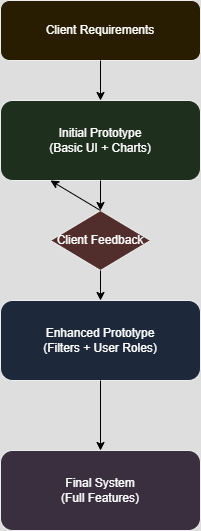
\includegraphics[scale=0.8]{Ch2/Prototype1.png}

\label{fig:Prototype Model}

% Diagram change as per your project demands

\section{Scope of Proposed System}
While in this phase, the scope of em was defined first and then what needs to be done was finalized. Lot of brainstorming ws were very clearly noted down. 
We never came back to revise or change the requirement defined earlier..............

\textbf{Advantages of Proposed System }\\


%\section{Hardware & Software Specifications}


% Write scope of your system.

\section{Technical Specification}
\textbullet \hspace{0.2cm} \textbf{Hardware Specification}\\
Processor	:	Intel(R) Core(TM) i3-7020U CPU @ 2.30GHz 2.30 GHz\\
RAM          	: 	Min. 2GB\\
Hard Disk	: 	Min. 20 GB free\\
% \textbullet \hspace{0.2cm} \textbf{Client}\\
% Processor   	: 	Intel(R) Core(TM) i3-7020U CPU @ 2.30GHz 2.30 GHz\\
% RAM           	: 	Min. 512 MB\\
% Hard Disk	: 	Min. 480 MB free\\
\textbullet \hspace{0.2cm} \textbf{Software Specification}\\
Platform	:  	Windows 11\\
Front End	: 	React.js, Redux (state management). \\
% Middle ware	: 	PHP (Framework : Codeigniter)\\
Back End	: 	Node.js, Express.js. \\	
Database    : MYSQL\\
Web Browser: 	Google Chrome etc. \\


% \subsection{Codeignitor Framework}
\subsection{Technology Stack Explained}
% CodeIgniter is a PHP-driven framework, you churning out dynamic, interactive, professional websites in no time.\\

% \textbullet \hspace{0.2cm}	It underpins the Model/View/Controller (MVC) approach to web development—a best practice philosophy all developers should adhere to.\\

% 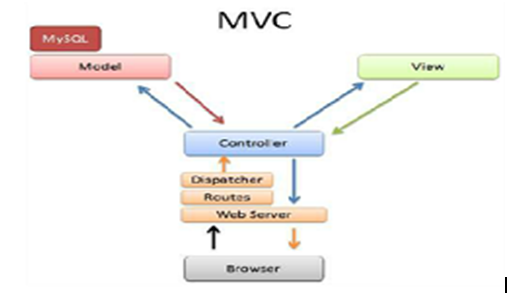
\includegraphics[scale=1.0]{Ch2/mvc.png}


% Diagram change as per your project demands (If required)
% \label{fig:MVC Model}

%\textbullet \hspace{0.2cm}It’s built on a linear, easy-to-use folder structure.\\


% This section type your project contents 
\begin{itemize}
    \item \textbf{\textcolor{techblue}{React.js}}: A JavaScript library for building dynamic, component-based user interfaces.
    
    \item \textbf{\textcolor{techblue}{Redux}}: State management tool to centralize and manage application data.
    
    \item \textbf{\textcolor{techblue}{Chart.js}}: Lightweight library for rendering responsive, interactive charts.
    
    \item \textbf{\textcolor{techblue}{D3.js}}: Powerful library for custom data visualizations using SVG/Canvas.
    
    \item \textbf{\textcolor{techblue}{MongoDB}}: NoSQL database for flexible, JSON-like data storage.
    
    \item \textbf{\textcolor{techblue}{Styled-components}}: CSS-in-JS library for scoped styling and theme support.
    
    \item \textbf{\textcolor{techblue}{Node.js}}: JavaScript runtime for scalable server-side execution.
    
    \item \textbf{\textcolor{techblue}{Express.js}}: Minimalist framework for building RESTful APIs and routing.
\end{itemize}
